\documentclass[12pt]{article}
\usepackage[margin=1in]{geometry}

\usepackage{color} % for highlighting

\usepackage{wrapfig}
\usepackage{graphicx}
\graphicspath{ {figures/} }
\usepackage{caption}    % to change caption font size
\captionsetup[figure]{font=footnotesize,labelfont=footnotesize}
\captionsetup[table]{font=footnotesize,labelfont=footnotesize}
\usepackage[above]{placeins} % for FloatBarrier

\usepackage{array}    % for table vertical align

\usepackage{enumerate}
\usepackage{enumitem}
\setlist{nolistsep}

\usepackage[numbers]{natbib}


\title{Understanding the Clinical Microbiome \\ Biological Engineering Thesis Proposal}

\author{Claire Duvallet}
\date{October 11, 2016}

\begin{document}


\maketitle
\newpage
\tableofcontents
\newpage
\begin{abstract}
In spite of the recent increase in research on the human 
microbiome, there is not a clear consensus on the relationship between 
human microbial communities and disease. Microbes colonize our entire bodies,
supplementing our body's functions, priming and training our immune 
systems, providing resistance to colonization 
by pathogens, and contributing to maintenance of health or progression of disease. 
However, major knowledge gaps exist in this field. 
The microbiota of some body sites have been much less studied than others.
Even extensively studied body sites lack a synthesized understanding of human-microbe-disease associations. 
Finally, interpreting exploratory microbiome analyses into biological hypotheses
remains challenging due to the lack of centralized tools and databases
for assigning biological traits to groups of microbes.

This thesis will expand our understanding of the clinical microbiome in three ways.
First, I will quantify the exchange between microbial communities
in the aerodigestive tract and investigate their associations with aspiration
and gastro-esophogeal reflux disease. 
This work will increase our understanding of the 
under-studied microbial communities of the aerodigestive tract.
Next, I will re-analyze published gut microbiome studies
across many disease states to identify disease-specific microbes
and shared microbial responses to disease.
No comparative studies currently exist which examine microbial communities
across a wide variety of diseases.
Finally, I will curate a database which links microbes to their biological traits, 
thus enabling generalizable interpretations of results from microbiome analyses.
Together, this work will contribute new knowledge
to the exciting field of human microbiome research and will 
empower researchers to draw clinically meaningful insights 
from their existing and future analyses.

\end{abstract}
\newpage

\section{Overall objectives and specific aims}
\subsection{Overall objectives}

The research presented in this thesis is united by a common purpose: 
advancing our understanding of the clinical human microbiome.
First, I will quantify the exchange across microbial communities
in the aerodigestive tract and examine their associations with clinical factors
such as aspiration and gastro-esophogeal reflux disease.
Second, I will re-analyze published gut microbiome studies in a 
broad comparative analysis. 
I will look for microbes which are frequently enriched or depleted
across many disease states as well as ones which are specifically 
altered in only one or two diseases. 
Finally, I will curate a database that annotates bacterial sequences 
with their associated biological traits. The information in this database will
be compiled by mining and combining existing literature, genomes, and datasets
related to the human microbiome.

\subsection{Specific aims}
\begin{description}
	\item[Aim 1] Apply standard methods to identify microbial 
	community characteristics associated with gastro-esophogeal reflux 
	disease and aspiration.
	\begin{enumerate}
		\item Quantify microbial exchange across sites in the aerodigestive 
		tract.
		\item Evaluate the effect of aspiration and gastro-esophogeal 
		reflux disease on aerodigestive microbial communities.
	\end{enumerate}
	\item[Aim 2] Re-analyze published gut 
	microbiome studies to identify disease-associated microbes and shared
	microbial responses to disease.
	\begin{enumerate}
		\item Compile and re-process publicly available case-control gut 
		microbiome studies with a standardized method.
		\item Identify generic microbial responses to disease shared across all studied disease states.
		\item Identify microbes consistently associated with specific diseases.
	\end{enumerate}
	\item[Aim 3] Curate a database of 16S sequences annotated with 
	associated general biological traits.
	\begin{enumerate}
		\item Combine existing databases and perform targeted literature searches 
		to annotate microbes based on known biological 
		traits.
		\item Use machine-learning techniques to extract disease-associated 
		groups of bacteria from datasets collected in Aim 2.
		\item Develop these microbial annotations into a collaborative 
		tool for use in interpreting new microbiome studies.
	\end{enumerate}
\end{description}
\newpage

\section{Background and significance}

The topics addressed in this thesis are connected by
the motivation to better understand
clinically-relevant associations between microbes and their human hosts.
My work will focus on the microbial communities of two major body systems:
the aerodigestive and gastrointestinal tracts. To study these, I will 
use a combination of traditional analytical techniques, supplemented by 
novel methods as required. This section will provide background on
the aerodigestive tract, the gut microbiome, and current analytical techniques 
used in microbiome studies. 

\subsection{Aerodigestive tract}

\subsubsection{Physiology and disease}

%\begin{figure}
\begin{wrapfigure}{R}{0.2\textwidth}
\begin{center}
    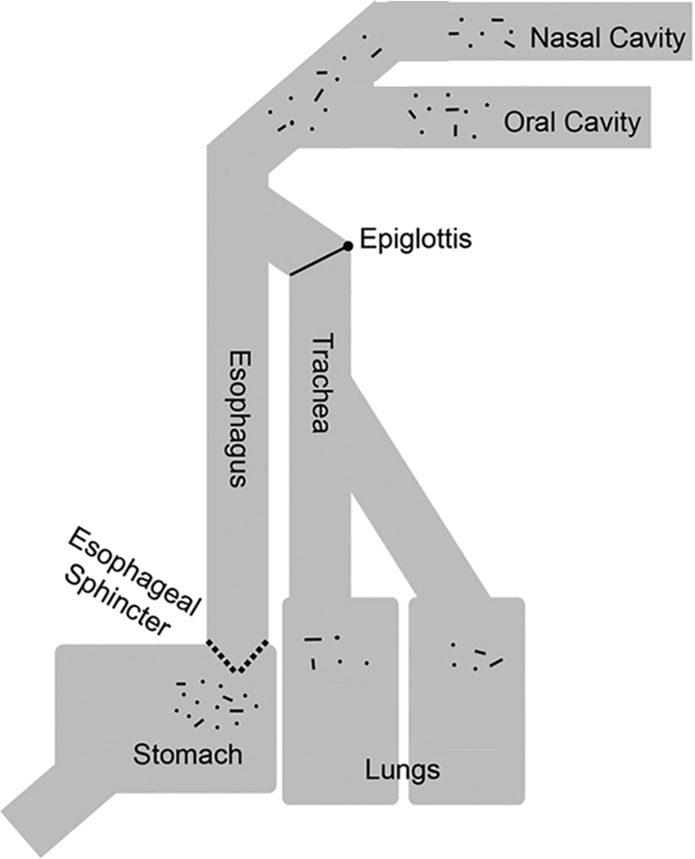
\includegraphics[scale=0.35]{aero_tract}
    \caption{Schematic of the flow relationship between sites of the 
    aerodigestive tract. Adapted from \cite{bassis-source-2015}.}\label{fig:aero_tract}
\end{center}
%\end{figure}
\end{wrapfigure}

From an engineering perspective, the aerodigestive tract,
consisting of the upper gastrointestinal and respiratory tracts,
can be thought of as different compartments connected by the esophagus and trachea (Figure \ref{fig:aero_tract}).
The mass transport between the throat, stomach, and lung compartments is regulated by complex physiological 
mechanisms. Swallowing guides material from the mouth to the stomach, 
but may dysfunction and allow material to enter the lungs. The 
esophageal sphincter usually prevents material from leaving the 
stomach, but sometimes allows gastric contents into the lungs \cite{beck-lung-2012}. Finally, complex 
homeostatic mechanisms clear the lungs of foreign bodies and create a 
selective environment for microbes in the lungs \cite{martinharris-mbs-2008, dickson-lung_microbiome-2014}. 
Understanding these complex physiological relationships is further complicated
by the experimental and ethical considerations related to the 
invasive sampling necessary to study the human aerodigestive tract \cite{beck-lung-2012}.

Gastro-esophogeal reflux disease (GERD) is a set of syndromes in which 
the reflux of stomach contents leads to troublesome symptoms or 
complications \cite{vakil-gerd_defn-2006, dent-gerd_epi-2005}. The most common symptoms of GERD 
are regurgitation and heartburn, but the disease may also present 
asymptomatically \cite{vakil-gerd_defn-2006, dent-gerd_epi-2005}. 
GERD can be diagnosed by demonstrating reflux of gastric contents, injury to the esophogus, 
or based on symptoms alone \cite{vakil-gerd_defn-2006}. GERD affects
10-20\% of people in Western Europe and North America, and can lead to severe complications such as Barrett's 
esophagus \cite{vakil-gerd_defn-2006}. Proton-pump inhibitors (PPIs) are often prescribed for GERD,
though long-term adverse effects of these drugs is becoming more widely understood \cite{sweet-gerd_asp-2009, imhann-ppi-2016, houghton-microaspiration-2016}.
In cases of severe reflux, fundoplication surgery may
be recommended, in which part of the stomach is wrapped around the 
esophagus to prevent refluxate from leaving the stomach and going up
into the esophagus \cite{sweet-gerd_asp-2009}. 

Aspiration is another complex aerodigestive condition in which foreign material is inhaled, either through macro-aspiration resulting from dysfunctional swallowing or micro-aspiration which is common in healthy people \cite{sweet-gerd_asp-2009, dickson-lung_microbiome-2014}.
Clinically, aspiration is defined as the inhalation of foreign material such as food or 
gastric contents into the lungs \cite{raghavendran-asp_injury-2011}. 
Most aspiration events are unwitnessed without obvious outward signs 
or symptoms, and may involved large quantities of aspirated material 
or may be micro-aspiration events \cite{raghavendran-asp_injury-2011}. 
Aspiration resulting from swallowing dysfunction can be diagnosed with 
a Modified Barium Swallow test (MBS) \cite{martinharris-mbs-2008}. In 
the MBS procedure, patients are observed videoradiographically as they 
swallow varying quantities and viscosities of food or liquid 
impregnated with barium, a contrast agent. The swallowing process is 
observed and abnormalities like aspiration of contents past the vocal 
chords can be diagnosed \cite{martinharris-mbs-2008, martinharris-clinical_mbs-2000}. 
However, the MBS test cannot be used to 
determine aspiration of gastric contents or episodes of micro-aspiration, which may also have clinical relevance 
\cite{raghavendran-asp_injury-2011, lee-pulm_asp-2014}. No validated clinical 
biomarkers exist to diagnose and define gastric and micro-aspiration 
events \cite{lee-pulm_asp-2014, debenedictis-asp_dis-2009}, but they are thought to play a role in 
causing or exacerbating many respiratory diseases 
\cite{houghton-microaspiration-2016, reen-aspirated_bile-2014, almomani-cf_sputum-2016}. Currently, microaspiration of gastric contents 
is studied by measuring the concentration of bile or pepsin in the 
lungs, but such assays are rarely validated against gold-standard 
methods and have not undergone clinical validation 
\cite{houghton-microaspiration-2016, lee-pulm_asp-2014}. Further complicating 
the issue is that many healthy patients have a baseline level of 
micro-aspiration \cite{dickson-lung_microbiome-2014, sweet-gerd_asp-2009, debenedictis-asp_dis-2009}.

GERD and aspiration are thought to be associated with many respiratory diseases, but the precise 
link and mechanisms underlying these associations remains very unclear 
\cite{houghton-microaspiration-2016}. The prevalence of GERD in 
respiratory diseases has been estimated to be up to 90\% for some 
diseases, and often presents without the common symptoms of heartburn 
or regurgitation \cite{houghton-microaspiration-2016}. Studies have 
shown that GERD is related to adverse outcomes after lung 
transplantation \cite{sweet-gerd_asp-2009} and reduced lung function in patients with 
cystic fibrosis \cite{almomani-cf_sputum-2016}. Aspiration of stomach 
contents is thought to contribute to these adverse outcomes, either 
through the aspiration of bile triggering a change in the lung's 
environment and making it more favorable to colonization, or through 
direct aspiration of gastric bacteria leading to infection 
\cite{reen-aspirated_bile-2014, almomani-cf_sputum-2016}. 
However, because of the difficulties in diagnosing and studying 
microaspiration, aspiration of gastric contents, and GERD, precise 
causal links between reflux, aspiration, and lung disease have yet to 
be established \cite{houghton-microaspiration-2016, debenedictis-asp_dis-2009, almomani-cf_sputum-2016}.

\subsubsection{Microbiome of the aerodigestive tract}
The microbial communities of the human aerodigestive tract are among the least 
studied human-associated microbiota. 
Neither gastric nor lung sites were included in the 
Human Microbiome Project, leading to a dearth of studies and data on 
these important body sites \cite{bassis-source-2015}. The lungs have classically thought to be sterile and free of bacteria in 
healthy people \cite{bassis-source-2015, beck-lung-2012, charslon-topographical-2011}. 
However, both culture-based
and culture-independent studies of the lung microbiome have recovered
bacteria, mostly of the \textit{Prevotella}, \textit{Veillonella}, and \textit{Streptococcus} genera \cite{bassis-source-2015}. 
Although the precise balance between factors that shape the lung microbiome 
remains to be fully elucidated, lung microbial communities are shaped by the balance of
immigration, elimination, and active colonization of microbes 
throughout the respiratory tract \cite{bassis-source-2015, dickson-lung_microbiome-2014}.
Existing studies have examined the microbiome of patients with cystic fibrosis, chronic obstructive 
pulmonary disorder, and asthma, as well as smokers and patients on PPI therapy 
\cite{almomani-cf_sputum-2016, rosen-ppi-2015, erbdownward-copd-2011}.
However, many of these studies are limited by small sample sizes due to the invasive 
nature of sampling human lungs. The stomach has also traditionally thought to be
relatively sterile due to its low pH \cite{lawson-gastric-2010}.
Many studies of the gastric microbiota have focused on \textit{Helicobacter pylori}, 
which colonizes many healthy patients and is also implicated in the development of gastric cancer and other stomach diseases \cite{bik-stomach-2006}.
These consistently find that \textit{Helicobacter pylori} dominates the mucosal 
community when it is present \cite{lawson-gastric-2010, bik-stomach-2006}.
Other culture-independent studies have found diverse gastric communities in 
both the mucosa and lumen of healthy patients' stomachs \cite{bassis-source-2015, rosen-ppi-2015, lawson-gastric-2010}.
While the majority of the gastric flora is likely seeded by the
oral microbiota (via swallowing), 
the stomach also contains its own unique community \cite{bassis-source-2015, lawson-gastric-2010}. 
Previous studies have examined the relationships between microbial communities in  the upper 
aerodigestive tract, with conflicting results \cite{bassis-source-2015, almomani-cf_sputum-2016, rosen-ppi-2015, charslon-topographical-2011}. 
Some have shown striking similarities in the microbial
communities across the respiratory tract \cite{bassis-source-2015, almomani-cf_sputum-2016} while others
argue that different sites have distinct microbial communities \cite{rosen-ppi-2015},
and that these vary even within individual sites like the lungs \cite{erbdownward-copd-2011, dickson-spatial-2015}.

\subsection{Gut microbiome}

\subsubsection{Gut microbiome in health and disease}

The human gastrointestinal tract is integral to health and disease
and its microbiota is, in turn, integral to its functioning.
The intestine digests food and absorbs nutrients, and  
also plays important roles in maintaining metabolic homeostasis, 
regulating hormone levels, and communicating sensory signals with the brain.
The microbes in our guts provide essential functions to our well being. 
They help us harvest energy from the food we eat and digest otherwise 
undigestible fibers, train our immune system, break down xenobiotics and 
other foreign products, and release metabolites and hormones that provide 
chemical signals to our body's regulatory mechanisms \cite{nash-baker, asd-kb, turnbaugh-energy_harvest-2006}. These signals can act locally in the gut 
and can also have larger systemic effects, for example by sending signals 
through the vagus nerve to the brain via the `gut-brain axis' \cite{asd-kb, asd-son}. 

Because of this complex interplay between host and microbes, many 
diseases have been hypothesized to be associated with the gut 
microbiome. These include metabolic disorders,
inflammatory and auto-immune diseases, pathogenic diarrhea, and others \cite{nash-baker, turnbaugh-energy_harvest-2006, edd-singh, par-schep}.
The relationship between the gut microbiome and obesity has been 
extensively studied in mouse models and human patients. These studies
have found encouraging results and causal associations in mice but 
relatively little consensus in humans \cite{turnbaugh-energy_harvest-2006, ridaura-mouse_fmt-2013, ob-escobar, walters-ob_meta-2014}. 
Related disorders like metabolic 
syndrome and diabetes have also been examined, with similarly little consensus on
specific microbial markers of these conditions \cite{mets-stad, ob-ross}. 
Inflammatory bowel disease (IBD) is a chronic disease characterized by 
mucosal inflammation of the gastrointestinal tract. Animal studies relating gut 
microbes, immune function, and IBD have pointed to an important role for 
bacteria in affecting the progression of IBD \cite{tamboli-ibd-2004}. 
Recent studies have focused on classifying IBD patients based on 
their fecal microbiota and on identifying discriminatory taxa in stool 
\cite{ibd-papa, ibd-gevers}. IBD patients have distinct microbial profiles 
that distinguish them from controls, but the specific microbes which
drive this distinction have not been identified, and it is likely that
larger community structure patterns play an important role in shaping
the IBD microbiota \cite{walters-ob_meta-2014, ibd-papa, ibd-gevers}.
Colorectal cancer (CRC) has long been associated with the intestinal 
microbiome, with bacterial metabolites thought to contribute to the 
development of CRC and specific bacteria having been isolated from CRC 
tumors \cite{crc_zeller, crc_xiang}. Studies have analyzed disease associations with 
tumor- and lumen-associated microbiota, and have consistently found 
enrichment of the \textit{Fusobacterium} genus in CRC patients
\cite{crc_zeller, crc_zhao, crc_zhu, crc_zackular}. 
Diarrheal diseases caused by intestinal pathogens have also been extensively 
surveyed using 16S methods, especially in the context of 
\textit{Clostridium difficile} infection (CDI) and related fecal 
microbiota transplants \cite{cdi_schubert, cdi_vincent}. Finally, diseases like rheumatoid 
arthritis, autism, Parkinson's, HIV, and others have also been 
examined for microbial associations, though these fields remain 
relatively unexplored \cite{asd-kb, par-schep, ra-littman, hiv-dinh}.

\subsubsection{Existing understanding of the gut microbiome}

Although specific microbiome-disease associations remain unclear, general characteristics
of the gut microbiome are relatively well-understood. People have their own unique gut microbial 
communities, very few microbes can be consistently found across the majority of people,
and many gut communities are dominated by one or two phyla (Bacteroidetes and Firmicutes) \cite{hmp-2012}.
Our gut microbiome is stable over time and can also change rapidly in response to 
disease, antibiotics, travel, and diet \cite{david-huge-2012}. These perturbations can be fully reversible
or can also have long-term effects \cite{david-huge-2012}.
Dysbiosis is often discussed as an ``imbalance'' of gut microbes, though
is generally applied to mean any community disruption related to disease \cite{costello-ecology-2012}.
Generally, less diverse communities are thought to be associated with disease,
though studies often find no significant association with diversity and disease \cite{walters-ob_meta-2014}.
Early mouse studies associated the ratio of Bacteroidetes to Firmicutes with
altered phenotypes, but few subsequent studies have found similar associations
in human patients \cite{turnbaugh-energy_harvest-2006, sze-signal-2016}. 

Combining existing studies to increase our ability to find consistent
disease associations is a promising approach, but existing meta-analyses
have had mixed results \cite{walters-ob_meta-2014, sze-signal-2016}. 
In some cases like IBD, strong and consistent 
signals can be found across studies but no specific microbes have 
been found to be consistently associated with IBD \cite{walters-ob_meta-2014}. Meta-analyses of obesity studies also tend 
to find no clear taxonomic associations with obesity \cite{sze-signal-2016, walters-ob_meta-2014},
even though the microbiome has been causally linked to obesity in mouse models \cite{turnbaugh-energy_harvest-2006, ridaura-mouse_fmt-2013}. 
Other meta-analysis studies are not relevant to extracting 
clinically-relevant microbial associations: many of these test the 
ability of various statistical and machine learning methods
to extract biomarkers or classify disease states, without much
interpretion of what the statistical results mean biologically
\cite{knights-supervised-2010, lozupone-meta-2013, knights-biomarkers-2011, pasolli-meta_analysis-2016}.

\subsection{Analytical background and significance}

\subsubsection{Data generation, standard analysis methods and associated challenges} 
A common way that researchers study the human microbiome is to do 
amplicon-based next generation sequencing of complex microbial 
communities. This culture-independent method begins with extracting
DNA from a sample of interest, amplifying the universally conserved
bacterial 16S rRNA gene, and sequencing by one of the available technologies such as 454 
Pyrosequencing or, more recently, Illumina HiSeq or MiSeq \cite{knights-supervised-2010, sze-signal-2016}. 
The resulting reads are quality-controlled and often processed into Operational Taxonomic Units (OTUs), 
clusters of similar sequences which serve as proxies for bacterial 
species \cite{knights-supervised-2010}. To interpret results, researchers assign taxonomies to 
OTUs using a variety of methods, for example by mapping them to 
annotated reference genomes or using a Bayesian classifier trained on 
a reference set of annotated bacteria \cite{wang-rdp-2007, mcdonald-gg-2011}. Each of 
these processing steps affects the eventual output data, and there
are no accepted standardized methods followed by all studies.

The data that results from these surveys can be very challenging to analyze.
The datasets are often very high-dimensional, with hundreds 
of OTUs present in a given cohort which may only have tens of samples \cite{sze-signal-2016}. 
The data is also incredibly sparse: only few OTUs tend to be 
present in many of the samples, and most entries in the data matrix 
are zeros \cite{knights-biomarkers-2011}. 
Furthermore, strong batch effects between studies result from 
differences in experimental and computational processing steps.
For example, different taxonomy databases contain different 
microbes or conflicting names for the same bacteria, making it 
difficult to compare even published results across studies.  
These issues may be large contributors to the lack of consensus on the 
role of the microbiome in disease, in spite of the broad availability of data and studies.

While there exist no established standards for processing or analyzing 
16S data, most researchers take similar approaches to gleaning insight 
from case-control cohorts \cite{knights-supervised-2010}. 
 Alpha diversity, the diversity of species within each sample, is usually compared across groups of interest. 
Beta diversity, the diversity between samples, is also frequently compared to understand whether 
samples within groups are more similar to each 
other than they are to the other group(s) \cite{knights-supervised-2010}. Finally, most studies perform 
univariate non-parametric tests on the abundance of OTUs to find 
bacteria significantly associated with the condition of interest \cite{wang-pval_method-2016}. 
However, because of the high-dimensionality of the data and the 
often very low sample sizes, many studies yield no significant
results \cite{wang-pval_method-2016}.

\subsubsection{Interpreting taxonomy-based microbiome analyses}\label{sec:gsea}
Few analytical tools exist to interpret the lists of
significant OTUs resulting from 16S analyses into biological hypotheses. 
When bacteria are found to be associated with the study condition of interest, 
identifying the patterns which group these bacteria 
together is a manual task for researchers. 
Typically, once significant OTUs are found for a certain condition,
researchers perform a literature search and hope to find 
previous reported associations or mechanistic studies on these bacteria.
Other more seasoned researchers can often look at a list and infer
over-representation of certain phenotypes, such as spore-formers
or upper gastrointestinal tract bacteria. However,
no tools providing a systematic approach to extract meaning from 
OTUs currently exist. Additionally, in many cases few or no OTUs are
found to be significantly associated with a condition of interest at all.

Enrichment analysis is a powerful way to directly identify biologically 
meaningful patterns in high-dimensional data. Enrichment analysis is 
widely used in RNA expression studies and has been proposed for use in 
metabolomics studies \cite{subramanian-gsea-2005, xia-msea-2010}. 
Gene Set Enrichment Analysis (GSEA) introduced
this statistical method to biomedical applications. In GSEA, genes are 
ranked by their differential expression between two conditions. Then, 
\textit{a priori}-defined groups of related genes are analyzed for 
over- or under-representation at either end of the ranked list. Rather 
than asking whether individual genes are correlated with a phenotype, 
GSEA allows for the identification of groups of genes which change 
together. This allows for identification of significant phenotypes 
where individual genes do not exhibit large enough changes to reach 
significance on their own. It also enables more direct biological 
interpretation, since the gene sets are defined \textit{a priori} 
based on biological knowledge. Enrichment analyses like GSEA
could be incredibly useful in microbiome studies, where 
many phenotype associations are likely to result from groups of
bacteria working together, and high-dimensional datasets
frequently produce few significant OTU-level phenotype associations.

Interpreting the biological significance of a list of significant OTUs 
through enrichment analysis relies upon the existence of trait annotations
for the OTUs in that list.
There currently does not exist a database which maps a microbe's
taxonomy (via its 16S sequence) to its biological traits.
In GSEA, genes were grouped into gene sets based on their common 
pathways, functions, locations in the chromosome, and associations 
with disease \cite{subramanian-gsea-2005}. 
Similar information exists for bacteria in some microbial databases, 
but none of these databases or tools have been combined to define groups 
of microbes based on their general traits. 
The Integrated Microbial Genomes \& Microbiomes (IMG) 
database contains approximately 10,000 annotated 
bacterial genomes, but the annotations are not fully complete and do 
not span all categories of interest \cite{markowitz-img-2013}. SourceTracker 
can be used to label microbial communities according to their 
environmental source, but requires input training sets with each use 
in order to learn the environmental associations and classify the input dataset \cite{knights-sourcetracker-2011}. 
Finally, bioinformatic tools like PiCRUSt have been developed that can infer functional 
content from 16S data \cite{langille-picrust-2013}, but these annotate
microbial communities with genes and KEGG pathways present in the communities
and do not necessarily translate these to generalizable biological traits.
Existing tools and databases for microbial annotations are often based either 
on inferences from genetic content or on experimentally validated phenotypes,
but rarely combine these two methods to create a comprehensive resource
that maps microbes to their varied biological traits.


\section{Research design and methods}

\subsection{Aim 1: Apply standard methods to identify microbial community characteristics associated with gastro-esophogeal reflux disease and aspiration}

The microbial communities of the lungs, stomach, and throat
are connected and likely exchange members, but the effects of GERD and aspiration 
on these microbial communities and their exchange are unclear \cite{bassis-source-2015}.
\textbf{We hypothesize that there is extensive microbial exchange occurring
across all sites of the aerodigestive tract, and that certain clinical conditions like aspiration
or GERD modulate the amount of exchange happening across various sites.}
To address this hypothesis, we will first identify which microbes
are exchanged across sites and define a metric to quantify this exchange. 
Next, we will investigate how aspiration and GERD affect aerodigestive microbial communities.
Aspirating patients are at a higher risk for respiratory
infections, and many patients who present with idiopathic
respiratory problems have a high prevalence of GERD \cite{houghton-microaspiration-2016,  debenedictis-asp_dis-2009}. 
Therefore, we hypothesize that aspiration will increase the microbial exchange between the lungs and the throat,
and that reflux will increase the exchange between the lungs and the stomach.
Quantitatively describing the amount of microbial exchange happening in the
aerodigestive tract and determining clinical modulators of this exchange
could inform treatments targeted toward reducing the exchange across specific sites.

\subsubsection{Aerodigestive patient cohort}

\begin{wraptable}{r}{5.8cm}
\begin{tabular}{l c}
	\hline
	\textbf{Sites} & \textbf{N} \\
	\hline
	gastric, throat, \& BAL & 87 \\
	gastric \& throat & 45 \\
	gastric \& BAL & 34 \\
	BAL \& throat & 9 \\
	\hline 
\end{tabular}
\caption{Number of patients with data for each combination of sites.}\label{tab:rosen_samples}
\end{wraptable}

The cohort presented in this work represents the largest collection of 
human aerodigestive tract samples of its kind.
It consists of 261 patients recruited by Rachel Rosen 
(M.D., GI/Nutrition) and her team at Boston Children's Hospital  
over the course of the past 6 years. Multiple samples were 
taken from patients: throat swabs, gastric fluid, and broncho-alveolar lavages (BAL) (Table \ref{tab:rosen_samples}). 
To acquire a BAL sample, a bronchoscope is inserted into the lungs 
of an anaesthetized patient, saline is flushed through the 
bronchoscope, and then suctioned back up \cite{charslon-topographical-2011}. 
Gastric fluid is suctioned during an endoscopy, and throat
swabs are acquired by brushing the posterior tongue \cite{rosen-ppi-2015}. 
Many patients in this cohort were monitored for GERD with 24-hour
impedance monitoring \cite{vakil-gerd_defn-2006}, which identifies the total number of reflux episodes,
the percent of time each patient was refluxing, and the acidic or non-acidic
nature of the reflux event. A subset were also tested for aspiration with
a Modified Barium Swallow (MBS) test.

\subsubsection{Quantify microbial exchange across sites in the aerodigestive tract} \label{sec:exchange}

To understand the microbial exchange between sites in the 
aerodigestive tract, we must first identify which microbes are being exchanged
and then quantify the extent of this exchange across the sites. 
\textbf{We define a microbe as exchanged between two sites if it has a significant, positive Spearman 
correlation of its abundance in both sites.}
In other words, if a microbe is consistently exchanged between sites, 
we expect that if we see little of it in one site in one patient, then we will also see little of it in the other site. 
If we see more of it in the first site in a different patient,
then we also expect to see more of it in the other site.
To calculate this correlation, we consider only patients who have the microbe present in both sites (blue points in Figure \ref{fig:sharedness_defn}).
\textbf{We quantify the extent of exchange, $p_s$ by determining what percentage of
patients are exchanging that microbe across their two sites.}
In other words, $p_s$  is the number of patients who have the microbe present in both 
sites divided by the total number of patients.
We will calculate this metric for each OTU across all site-combinations, 
i.e. throat and lung, stomach and lung, and stomach and throat.

One factor to consider when drawing conclusions from the $p_s$ metric 
is that because of the low bacterial biomass in the gastric and lung 
sites, it is possible that some microbes which are ``exchanged'' across 
these sites are simply both being seeded by the environment. However, 
if these microbes are phylogenetically related or if they are known 
members of the gastric or lung communities, this would indicate that 
the OTUs are being selected for by the environment and are relevant 
community members. If exchanged microbes are closely related, this
would indicate either non-random seeding of the aerodigestive communities 
or non-random selection of randomly-seeded microbes. In either case, the
identified microbes would be a relevant part of the microbial communities.
Also, we can compare the exchanged OTUs we identify with previous work
to determine whether these microbes could be considered commensals or
if they have functions that would allow them to survive in their specific niches.

%\begin{wrapfigure}{R}{0.5\textwidth}
%	\centering
\begin{figure}
\begin{center}
    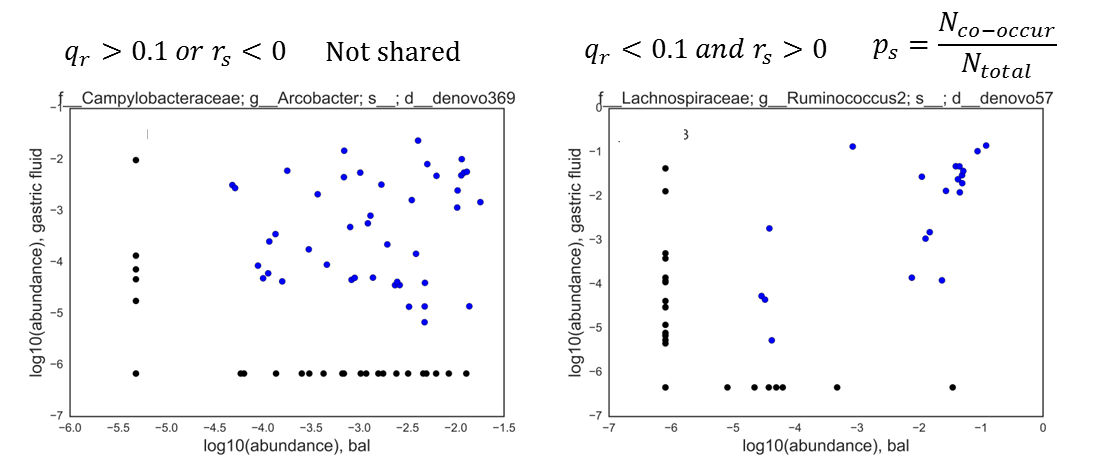
\includegraphics[scale=0.75]{sharedness_definition}
    \caption{If the abundance of a microbe when it is 
    present in both sites is significantly positively correlated, then we consider it exchanged 
    across those sites (blue points, right panel). $p_s$ is then calculated as the 
    percentage of patients who have the microbe present in both sites (blue 
    points divided by total points, where each point represents one patient). 
    Example of microbes which are (A) not exchanged and (B) exchanged between the 
    stomach and lungs.}\label{fig:sharedness_defn}
\end{center}
\end{figure}
%\end{wrapfigure}

\subsubsection{Evaluate the effect of aspiration and gastro-esophogeal reflux disease on aerodigestive microbial communities}

Once we quantify microbial exchange within the aerodigestive tract, we 
can begin to ask how conditions like aspiration and GERD modulate the exchange 
that occurs between them. \textbf{Our first hypothesis is that aspirators will have more exchange between their throat 
and lungs than non-aspirators.} Because aspirators cannot reliably protect
their airways from foreign materials in general, they may also have more exchange between their stomachs and lungs.
Aspirating patients are at higher risk for respiratory infections, which
may be a result of stomach or oral microbes successfully seeding the lungs
because the airway is no longer adequately protected.
Reflux surgery is often prescribed to aspirators with chronic infections,
as it is thought that the refluxate of these patients carries microbes which seed the lungs. 
Identifying how the throat-lung and stomach-lung connections are affected by aspiration 
would shed light on the involvement of the microbiota in these two clinical hypotheses.
The dataset has 48 patients with abnormal MBS test results (aspirators) and 63 patients with normal results.

\textbf{Our next hypothesis is that patients with more severe GERD will have 
more exchange between their stomach and lung communities.} Because we are 
interested in GERD that may modulate the stomach-lung connection, 
we will focus our analyses on full-column reflux, i.e. reflux that reaches the 
proximal (top) part of the esophagus, since it is more likely to enter the lungs.
Our GERD data quantifies the
percent of reflux which is full-column, but does not provide a hard
cutoff above which reflux is considered ``severe''. Thus, a secondary goal
of this work is to identify if such a threshold exists. We will examine
how exchange between and similarity of the lung and gastric communities
changes as a function of the ``severity'' cutoff. If we find a cutoff
in which the amount of exchange in patients who are above the cutoff is 
significantly higher than in patients who are below the cutoff, then perhaps
this threshold could define the clinically-relevant amount of reflux that is
problematic. The dataset has 125 patients with reflux testing.

For each of these clinical factors, \textbf{we will compare the amount of microbial
exchange occurring between the sites of interest in the two groups of patients},
i.e. non-aspirators vs. aspirators or less severe reflux vs. severe reflux. 
We will calculate a new $p_s$ within each patient 
subgroup for each of the previously-defined exchanged microbes.
In other words, $p_s'$ will be the percentage of the patients in one subgroup
that have the exchanged microbe present in both of their sites.
\textbf{We will also investigate how community similarities across aerodigestive
sites are affected by the conditions.} We will calculate the beta diversity
between the two sites for each patient who has sequencing data for both of
the sites. If a clinical factor increase the amount of exchange between
two sites, we expect to see either more exchange of specific microbes 
and/or more similar overall communities across the two sites.

An important consideration when interpreting these results is that
this work does not address the direction of microbial exchange between 
aerodigestive sites, nor does it directly link increased microbial 
exchange with adverse outcomes like respiratory infections.
We assume that most of the downstream communities are being seeded from the throat, 
but do not explicitly know the balance between immigration, elimination, and 
growth of microbes in each site \cite{bassis-source-2015}.
Follow up studies focusing on patients who develop respiratory 
infections or who frequently have GERD- or aspiration-associated 
respiratory infections should be undertaken to directly link the exchange
between communities with subsequent adverse clinical outcomes. 

\subsection{Aim 2: Re-analyze published gut	microbiome studies to identify disease-associated microbes}\label{sec:aim2}
Many researchers have found associations between gut microbial 
communities and individual diseases, but combining results from 
different studies about the same disease often yields conflicting results. To date, no one has
performed a comprehensive comparison of the results from gut microbiome 
studies across all disease states with standardized processing
and analysis methods.
\textbf{We hypothesize that re-analyzing existing gut microbiome datasets 
across all diseases will identify bacteria
associated with a general response to disease
and others associated with specific disease states.}
To address our hypotheses, we will first acquire and re-process a comprehensive
collection of case-control gut microbiome datasets. 
We will perform univariate tests for 
microbial associations with disease in each individual dataset. 
We will then combine the results from these univariate analyses across all datasets and,
separately, across all datasets of the same disease \cite{zavkin-ztest-2011}.
Microbes which are significantly enriched or depleted across 
all datasets will be considered part of a shared microbial response to
disease, whereas those which are only associated with one or two
individual diseases will be considered putative microbial markers of those diseases.
These findings will increase our understanding of
the role that microbial communities play in maintaining health or promoting disease,
point to potential biomarkers for specific diseases,
and motivate future mechanistic studies on the relationship between microbes and their human hosts.

\subsubsection{Compile and re-process publicly available case-control gut microbiome studies}
\textbf{To perform a meta-analysis, we will first collect a 
comprehensive selection of 16S gut microbiome case-control studies}. We 
will identify these studies through a targeted literature search.  
Inclusion criteria for datasets is ones which contain 
16S rRNA sequences from human stool samples with at least 15 patients in the
case (i.e. disease) group. Studies which focus exclusively on 
children under 5 will be excluded from these analyses, as the infant
gut microbiome does not resemble that of adults \cite{lozupone-meta-2013}.
We will also consider only datasets with 
publicly-available data, either from data repositories like SRA or
from personal email communication with authors. We will not 
apply for special permissions to use IRB-protected data. 

\textbf{We will process these datasets using a standardized in-house pipeline} 
developed by Thomas Gurry, a post-doc in the Alm lab. We will 
start with the least processed data available - in most cases, these will be 
raw FASTQ files but for some studies we will begin from quality-filtered 
FASTA files. Sequences will be quality and length trimmed, clustered 
at 100\% similarity, and assigned Latin taxonomic names using the RDP 
classifier \cite{wang-rdp-2007}. Samples with fewer than 100 reads will be removed from 
consideration. OTUs with fewer than 10 reads or which are present in 
less than 1\% of samples will be removed. More stringent quality 
filtering may be considered in order to reduce noise in the dataset.

Different studies sequence different regions of the 16S gene,
preventing us from using open-reference OTU sequences to compare
microbes across studies. Therefore, we will collapse OTUs
based on their taxonomic assignment and compare these across studies.
Analyzing OTUs at the species or strain level would be ideal,
but 16S data is limited in that most OTUs cannot be classified
down to such taxonomic resolution. On the other hand, the majority of gut microbiome
OTUs tend to be classifiable to genus level. Thus, collapsing to the genus level 
provides a good balance between the taxonomic resolution we can get with the 
amount of data we have to discard (i.e. unannotated OTUs).
Additionally, previous work has found that the maximal predictive power of the microbiota
to distinguish between different phenotypes
occurs at various taxonomic thresholds \cite{knights-biomarkers-2011}, so we will
also consider higher-level taxonomic classifications in our meta-analyses.

\subsubsection{Identify generic microbial responses to disease shared across all studied disease states}\label{sec:indep_studies}
Once we re-process existing
gut microbiome datasets in a standardized way, \textbf{we hypothesize that we
will identify broad community shifts related to generic disease.}
We will begin by comparing summaries of the microbial communities in 
each disease state. For example, we will compare the differences in alpha diversity 
for all cases and controls of the same disease across multiple datasets. 
We can combine alpha diversities from different studies in two ways.
First, we can standardize the alpha diversities within each study
(i.e. by subtracting the mean and dividing by the standard deviation), combine samples from
studies focused on the same disease, and perform a statistical comparison of
the alpha diversity across all samples in the case or control groups.
 Alternatively, we can
do individual statistical comparisons within each study and combine these p-values
together with the weighted Z-test, a method used in meta-analyses for combining p-values \cite{zavkin-ztest-2011}. We will begin with alpha diversity
because it is the most frequently reported metric in the microbiome literature. We will also similarly consider
other community summaries like the Bacteroides/Firmicutes ratio, beta diversity between and within cases and controls, 
and phyla abundances.

\textbf{We also hypothesize that certain microbes are part of a shared response to disease.} We will use univariate non-parametric statistics to compare the
abundance of individual microbes between cases and controls. 
To compare microbes across disparate studies, we will analyze OTUs
that have been collapsed to the genus level.
We will combine the univariate results across all studies using 
the weighted Z-test \cite{zavkin-ztest-2011} to determine the overall significance
of each microbe across all diseases. 
Genera which are significant after multiple hypothesis corrections
and meta-analysis combination are those which can be considered
to contribute to general phenotypes of health (if they are
consistently more abundant in controls) or disease (if they are
consistently more abundant in cases). We will also look for
similar consistent associations with higher-order taxa, in order
to identify whole clades of related organisms which are 
associated with health or disease.

\subsubsection{Identify microbes consistently associated with specific diseases}
\textbf{Next, we aim to identify microbes which are consistently associated with \textit{specific}
diseases.} We will
combine univariate results for individual diseases by 
using the same meta-analysis method described above, but now only
combining datasets which analyze the same individual disease state \cite{zavkin-ztest-2011}. 
We expect to find two types of disease-specific microbes from this analysis.
The first is bacteria which are not part of the generic response to 
disease but which are significantly enriched or depleted in 
an individual disease state.
The second is bacteria which \textit{are} enriched or depleted in the generic
response to disease, but which have a different directionality
in a specific disease. For example,
a microbe could be significantly depleted overall across all studies,
but significantly enriched when looking just within the obesity studies.
The microbes we identify with this
analysis may be very interesting candidates for biomarkers or mechanistic follow-up studies.

In this aim, we may struggle to find bacteria consistently 
associated with diseases because of technical batch effects, even 
where we expect to find a clear signal (i.e. in diseases which have 
had clear results from experimental or mechanistic studies \cite{turnbaugh-energy_harvest-2006, ridaura-mouse_fmt-2013, crc_zeller}). 
Developing robust methods to overcome technical batch effects in 16S 
studies is not within the scope of this work, but there are many
simpler options available to help mitigate batch effects. 
First, we can apply simple linear correction methods 
like subtracting the principal components of variation which correlate closely with technical 
artifacts like read depth or sample size. 
Another option is to use open-reference OTUs rather than collapsing to genus
and compare the phylogenetic relationships of the significant OTUs across different studies. 
Finally, we could also approach our meta-analysis from a functional point of view by
using tools like PiCRUSt to assign functionality to our
observed taxonomies \cite{langille-picrust-2013}.

%\subsubsection{Identify relationships between physiologically-related diseases by comparing their microbial characteristics}\label{sec:signatures}
%We also hypothesize that similar diseases will have similar 
%microbial community disruptions. For example, we expect that metabolic 
%diseases like obesity and diabetes will have more similar microbiota 
%changes to each other than they will to diarrheal diseases like \textit{Clostridium 
%difficile} infection or enteric diarrhea. We will summarize each 
%dataset with one vector indicating its ``microbial signature''. This 
%signature will include the number and identities of microbes 
%significantly associated with the disease and the direction of change 
%of these microbes relative to the controls. Depending on the results from Section 
%\ref{sec:indep_studies}, we may also include factors like differences 
%in alpha diversity or Bacteroides/Firmicutes ratios. Then, we will 
%investigate which datasets cluster together in this ``signature space'' 
%to identify those which have similar microbial characteristics (Figure \ref{fig:microbe_signatures}).
%
%%\begin{wrapfigure}{R}{0.5\textwidth}
%%	\centering
%\begin{figure}
%\begin{center}
%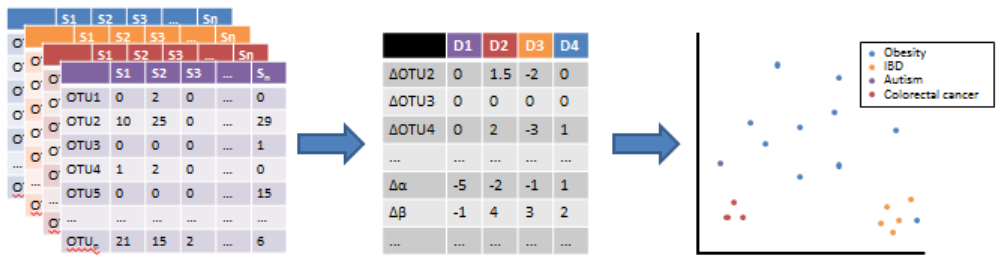
\includegraphics[scale=0.4]{microbial_signatures}
%\caption{We will define a microbial signature for each dataset by summarizing
%the association of each of its OTUs with the disease of interest. We will
%also include other relevant features like alpha and beta diversities. These 
%signature vectors will be used to cluster datasets and analyze resulting patterns.}\label{fig:microbe_signatures}
%\end{center}
%\end{figure}
%%    \caption{Defining microbial signatures}
%%\label{fig:microbe_signatures}
%%\end{wrapfigure}
%
%If a disease has a strong impact on or association with the gut 
%microbiome, then we would expect the signatures from multiple studies of that disease
%to cluster very tightly together. If this is the case, we can extract 
%the bacterial features which contribute the most to this tight 
%clustering - these will then be most likely to be associated with that 
%specific disease, and would be good candidates for further mechanistic 
%explorations. On the other hand, if datasets of the same disease or 
%similar conditions do not have similar microbial signatures, this may 
%indicate that the microbiome is not inherently implicated in or significantly affected 
%by that condition. In this case, the signal that we see in the gut 
%microbiome is likely driven by other non-disease effects, which are 
%not necessarily the same across studies. Alternatively, these diseases
%may have small biological signals which are dwarfed by batch effects
%between studies. Finally, if we find different 
%diseases with similar underlying causes (i.e. inflammation) clustering 
%near each other, then perhaps this would indicate that the microbiome 
%is affected or involved with the underlying cause rather than the 
%specific diseases. Such insights could help us design better 
%experiments to follow up on mechanism or causal relationships between microbes
%and disease.

\subsection{Aim 3: Curate a database of 16S sequences annotated with general biological traits}
Microbiome studies yield associations between
16S sequences and disease, but many of these sequences
do not have functional annotations in existing databases. Tools that connect
unannotated sequences to functions do not include
general biological traits, making it difficult to interpret
results from microbiome studies into biological hypotheses.
\textbf{In this aim, we will develop a centralized database of 16S sequences annotated with 
their associated biological traits.}
We will begin
by searching the literature for existing databases, combining their annotations and supplementing them
with literature search and genome-mining as needed. 
We will begin with traits like
sporulation and body site habitat. We will also
include disease associations that we identified in Aim 2 and search
for other putative phenotype-associations in these datasets.
Finally, we will package our database into a tool that researchers can use
to interpret their case-control microbiome studies into biological hypotheses and possible mechanistic associations. 

%lists of many microbes significantly
%associated with the disease states or conditions of interest. 
%Generating biological or mechanistic hypotheses based on these lists of 
%microbes currently relies mostly on searching existing literature for similar
%previously reported associations. 
%However, the vast diversity of microbes and the lack of standard
%processing or analysis methods makes it difficult to extract overall
%biological patterns from the published literature.
%Furthermore, the majority of 16S sequences in our databases do not have functional 
%or trait-based annotations, leaving researchers with few tools to 
%assign general biological interpretations to the results of their microbiome analyses.


%	\item[Aim 3] Curate a database of 16S sequences annotated with 
%	associated general biological traits.
%	\begin{enumerate}
%		\item Combine existing databases and perform targeted literature searches 
%		to annotate microbes based on known biological 
%		relationships.
%		\item Use machine-learning techniques to extract disease-associated 
%		groups of bacteria from datasets collected in Aim 2.
%		\item Develop these microbial annotations into a collaborative 
%		tool for use in interpreting new microbiome studies.

\subsubsection{Combine existing databases and perform targeted literature searches to annotate microbes based on known biological traits}\label{sec:set_curation}

In order to begin curating our database of microbes and their traits, 
\textbf{we will perform an extensive literature search
to identify existing databases and comprehensive review papers with experimentally 
validated microbial phenotypes}. We will combine these databases
and identify where they are missing annotations.
We will begin with IMG, a database with approximately 10,000 annotated microbial genomes. 
About half of these genomes are human-associated bacteria, 
and half of those have annotations for traits like disease 
association, sporulation, and body site habitat. 
We will extract the 16S sequences for the microbes in this database
and ensure that all of the organisms we identified in Aim 2
are represented in IMG's annotated microbes. If specific microbes are missing from IMG,
we will manually include them and their associated metadata from NCBI queries 
and targeted literature searches.

In collaboration with Ilana Brito, Assistant Professor of Biomedical Engineering at Cornell University, 
\textbf{we will apply a combination of literature mining and bioinformatics approaches to fill 
out the missing annotations in the databases and to add our own traits
of interest} (Figure \ref{fig:microbe_sets}). 
For example, in order to annotate spore-forming microbes, we will first perform a literature
search to identify known sporulation genes. We will then search for these genes in 
the whole genomes of representative organisms or in the 16S-based functional
profiles inferred by PiCRUSt \cite{langille-picrust-2013}.
Organisms which have these genes will be annotated as spore-formers. 
As another example, annotating traits like body site habitat will 
depend mostly on literature search since there are likely no clear genes
conferring this trait. We will also extract habitat associations
from large datasets like the Human Microbiome Project which sequenced multiple body sites \cite{hmp-2012}.
Throughout our annotation process, we will need to balance
the confidence we have in the annotations with
the breadth of microbes we are able to annotate.
For example, some bacteria which are known spore-formers do not contain any
known sporulation genes. We will fill these out to the best of the field's
existing knowledge, but our database will certainly 
still contain a vast number of false negatives.
On the other hand, microbes which have certain sporulation genes
may not express them in a biologically meaningful way in the human-associated
environment. Therefore, it will be important for our database to include information
on how the annotations were derived, i.e. from experimental studies, genetic content 
inference, or taxonomy-based functional inferences.

\begin{figure}
\begin{center}
	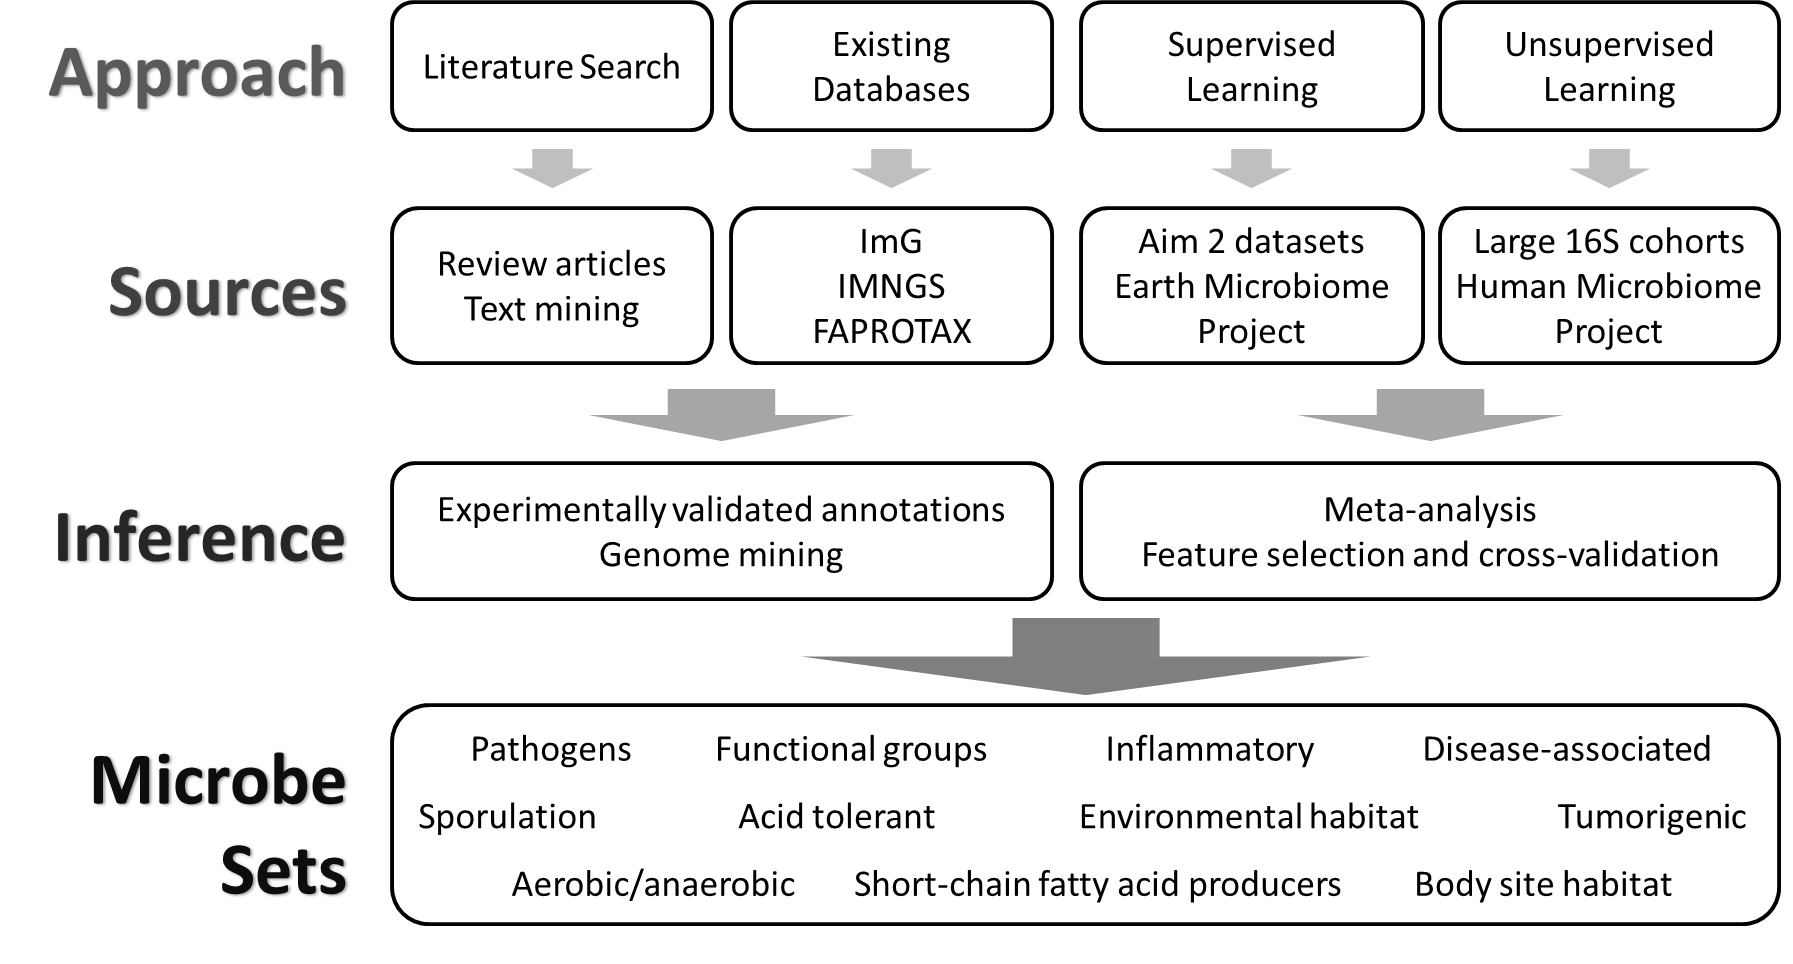
\includegraphics[scale=0.4]{microbe_sets}
	\caption{A variety of approaches will be used to define
	microbe sets, including manual curation from literature
	and database searches and data-driven methods (``Approach'').
	Many different kinds of resources will be drawn upon 
	(``Sources'') to infer groups of related microbes 
	(``Inference'') based on different categories 
	(``Microbe Sets''). Databases described in \cite{markowitz-img-2013, louca-faprotax-2016, lagkouvardos-imngs-2016}}
	\label{fig:microbe_sets}
\end{center}
\end{figure}

\subsubsection{Extract disease-associated groups of bacteria from datasets in Aim 2}
\textbf{In parallel with our literature-based annotations, 
we will use the datasets collected in Aim 2 to identify
additional disease-associated groups of microbes.} We will annotate microbes 
based on whether they were enriched or depleted in the shared microbial response to disease or if they were associated with specific diseases. 
We will also extract additional disease- and phenotype-associated microbes by 
applying machine learning methods to the datasets in Aim 2 for
various classification tasks (Table \ref{tab:classifications}). 
We will consider only genera which were present in the majority of studies 
in order to both reduce the dimensionality of the classification 
task and also ensure that extracted groups of microbes
are likely to be generalizeable to future studies. Random forest (RF) and support
vector machine (SVM) classifiers are the most commonly used methods in
microbiome studies and have been shown to perform well in discriminating
phenotypes based on 16S data \cite{ibd-papa, knights-supervised-2010, pasolli-meta_analysis-2016}. 
We will apply these methods to various classification tasks (Table \ref{tab:classifications})
and identify the most important features (RF) or those with the highest support (SVM)
for each successful classification.
Cross-validating the extracted feature sets across different datasets with the same
classification task will ensure the general discriminatory 
power of those microbes and prevent over-fitting.

These approaches may yield few or no groups of microbes with phenotype associations
that we are confident enough in to include in our database.
Considering the diversity of the gut microbiome across people and the
sparsity and high-dimensionality of 16S data, 
this result would not be surprising and underscores the importance of the
manually supervised curation work described in Section \ref{sec:set_curation} \cite{knights-biomarkers-2011, wang-pval_method-2016}.
If this happens, we will investigate higher-order taxa as possible features,
as this will reduce the dimensionality, sparsity, and inter-personal 
variability in the datasets.
Another approach is to directly convert each 16S community to functional profiles \cite{langille-picrust-2013}, perform feature selection on these functional community profiles, and then
convert these selected functions into taxonomically-defined groups of microbes. 
We could convert discriminatory functions back to taxa
by either identifying the bacteria which most frequently have
the discriminating function(s) in the datasets of interest, or by identifying all bacteria which have that function across all datasets.
{
\renewcommand{\arraystretch}{1.2}
\begin{table}
\begin{center}
\begin{tabular}{ m{6cm} m{10cm} }
	\hline
	\textbf{Microbe set association} & \textbf{Classification task} \\
	\hline
	General health/disease & All healthy vs. all disease \\
	%\hline
	Diarrhea & CDI, EDD, IBS-D vs. controls \\
	%\hline
	Neurological & Autism, Parkinson's vs. controls \\
	%\hline
	Liver & NASH, MHE vs. controls\\
	%\hline
	Metabolic syndrome & T1D, T2D, obesity, metabolic syndrome vs. 
	controls \\
	%\hline
	Autoimmune/inflammatory & T1D, rheumatoid arthritis, psoriatic arthritis, Crohn's disease 
	vs. controls or non-autoimmune patients \\
	\hline
\end{tabular}
\caption{Classification tasks to identify groups of phenotype-associated microbes.}\label{tab:classifications}
\end{center}
\end{table}
}
\subsubsection{Develop collaborative tool for interpreting microbiome studies}
\textbf{We will make our microbial trait annotations available to researchers as both
a flat database and as a packaged tool to interpret
16S studies.} Through our literature searches, 
we will identify the format of databases that researchers have found most 
useful and strive to package our annotations in a user friendly, useful format. 
We will likely begin with one very large text file containing all of 
the microbes, 16S sequences, and trait annotations that we have gathered. In addition to distributing the annotations themselves, we will also package them into a tool 
that researchers can use to interpret their 16S 
studies. Our software will take as input an OTU table and labels for different categories
of samples (i.e. cases and controls). 
It will perform enrichment analysis on the OTU table and return the 
results to researchers, similar to the Broad's Gene Set Enrichment Analysis tool \cite{subramanian-gsea-2005}. All of this work will be done using public open-source tools like 
GitHub to encourage collaboration and dissemination of our findings.

Developing a database of microbial annotations is a daunting task due 
to the vast diversity and complexity of microbes. We recognize the 
inherent difficulty of this task, and do not expect to produce a fully 
comprehensive database. However, because our annotations are intended 
to serve as a tool for biological interpretations and hypothesis 
generation, even a partially-complete database will be extremely 
valuable in reducing the number of false-negative results in microbiome 
studies. It will also be immensely useful
to researchers by providing coherent biological interpretations 
of existing results. We also recognize that our work will contribute to the 
beginning of a systematic grouping of phenotypically-associated 
microbes, and so we will ensure that the architecture of our database and annotation tool 
is easily accessible and modifiable by other researchers.


\section{Preliminary studies}

\subsection{Aim 1: Aerodigestive microbiota associated with GERD and aspiration}

\subsubsection{Aerodigestive communities exchange microbes across all sites}

We identified over 150 OTUs exchanged across sites in the aerodigestive tract 
(Appendix \ref{sec:appendix_figures}, Figure \ref{fig:shared_phyla})
using our definition of $p_s$ (Section \ref{sec:exchange}).
As expected, the majority of exchange occurred between the throat and stomach \cite{bassis-source-2015}.
Interestingly, the stomach and lung communities were almost as similar to
each other as the throat and stomach communities were,
but had less frequent exchange of specific microbes (Figure \ref{fig:similarities}). 
These findings support the hypothesis that frequent non-specific microaspiration
of gastric contents into the lungs is occurring,
in which the exchange of microbes is more stochastic and
not necessarily consistently selecting for specific community members across many patients.
Finally, we observed a decreasing trend in number of exchanged microbes 
across throat and stomach, lung and stomach, and throat and lung sites, respectively, 
for all phyla except Proteobacteria (Appendix \ref{sec:appendix_figures}, Figure \ref{fig:shared_phyla}). 
More Proteobacteria OTUs were exchanged 
between lungs and stomach than between the throat and stomach. Proteobacteria are 
known aerobes, and so may be preferentially selected for colonization in 
the lungs after microaspiration from the stomach.
These results support the existing hypothesis that the majority of
exchange across aerodigestive sites occurs between the throat and stomach, and
also shows that stomach and lung communities may be more related than previously
thought.

\begin{figure}[h]
\begin{center}
	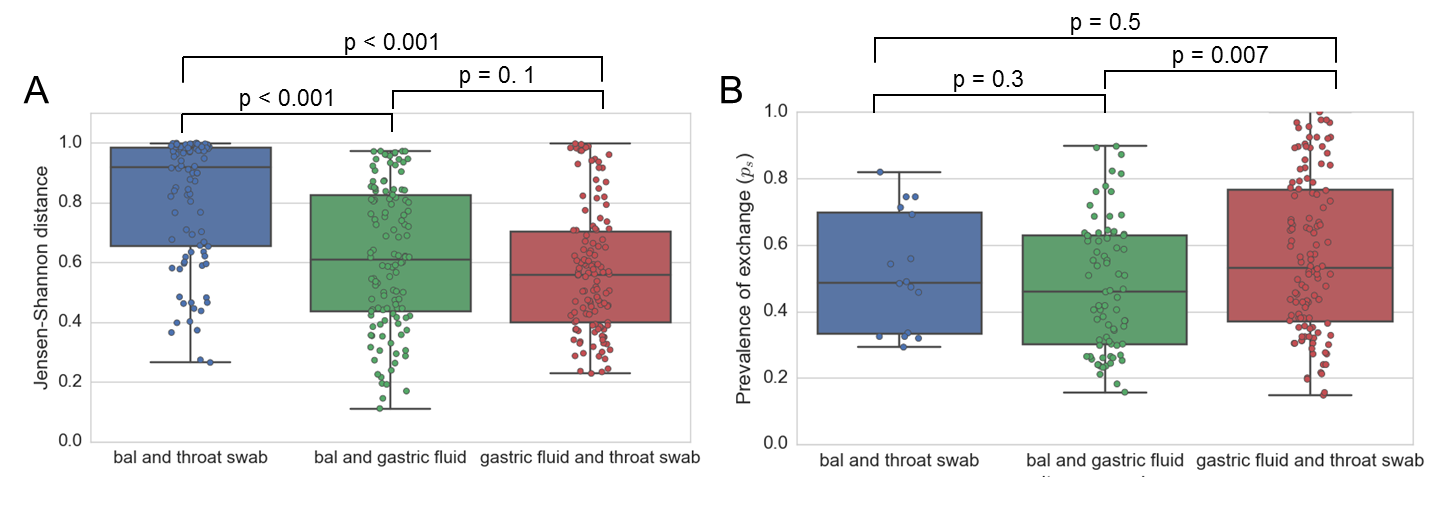
\includegraphics[scale=0.6]{all_jsd_sharedness}
	\caption{Community similarities and exchange across sites.
	(A) Jensen-Shannon distance (JSD) between sites within each patient. 
	Identical communities have a JSD = 0; completely different
	communities have JSD = 1. (B) $p_s$ for each exchanged OTU across 
	all site combinations. P-values calculated with a
	non-parametric Kruskal-Wallis test.}
	\label{fig:similarities}
\end{center}
\end{figure}

\subsubsection{Aspiration increases throat-lung exchange and gastro-esophogeal reflux affects stomach-lung relationship}

We observed a distinct increase in the amount of exchange between the 
throat and lungs of aspirators relative to non-aspirators (Figure \ref{fig:aspirators}B).
40\% of aspirators shared
the previously-defined throat-lung microbes between their throats and lungs, while only 15\% of 
non-aspirators did. Additionally, the throat and lung communities
were significantly more similar in aspirating patients than non-aspirators (Figure \ref{fig:aspirators}A). These results indicate that a consequence of abnormal swallowing
dysfunction is likely a seeding of the lungs with oral bacteria.
Interestingly, the stomach and lung communities of aspirating
patients were slightly more similar to each other than in non-aspirators, but not significantly so.
This indicates that the stomach is not likely a major source
of bacterial seeding of the lungs, even in aspirators. One of the current treatments for
aspirating patients who have frequent respiratory infections is fundoplication,
an invasive surgery that prevents refluxate from exiting the stomach, because it is thought
that the bacteria in the refluxate is seeding the lungs
and resulting in infection.
These findings show that fundoplication surgery may not be the best course of action in aspirators, since 
the bacterial exchange between stomach and lungs is not
significantly different from the exchange in normal patients \cite{debenedictis-asp_dis-2009, kawahara-fundo-2004}.

\begin{figure}[h]
\begin{center}
	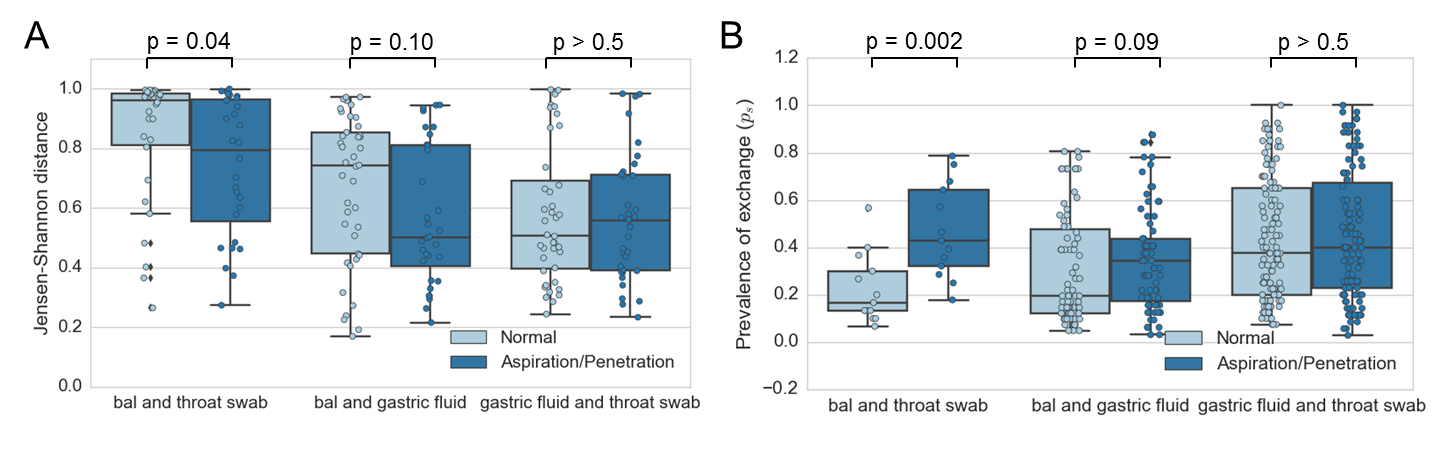
\includegraphics[scale=0.65]{aspiration}
	\caption{Community similarities and exchange across sites, stratitified by aspiration status.
	(A) and (B) as in Figure \ref{fig:similarities}.}
	\label{fig:aspirators}
\end{center}
\end{figure}

As expected, stomach and lung communities of patients with severe reflux were
more similar to each other than in patients without
severe reflux (Figure \ref{fig:reflux}A). 
Interestingly, patients with severe reflux were not more likely
to exchange the previously-defined stomach-lung microbes between their stomachs and lungs (Figure \ref{fig:reflux}B).
In this work, `severe reflux' was defined as reflux in 
which more than half of events were full-column events.
Future work will determine the effect of this `severity' 
threshold on the amount of exchange, with the aim
of identifying whether a severity threshold exists above which bacterial exchange
between the stomach and lungs becomes significantly higher than in non-severe reflux patients.

\begin{figure}[h]
\begin{center}
	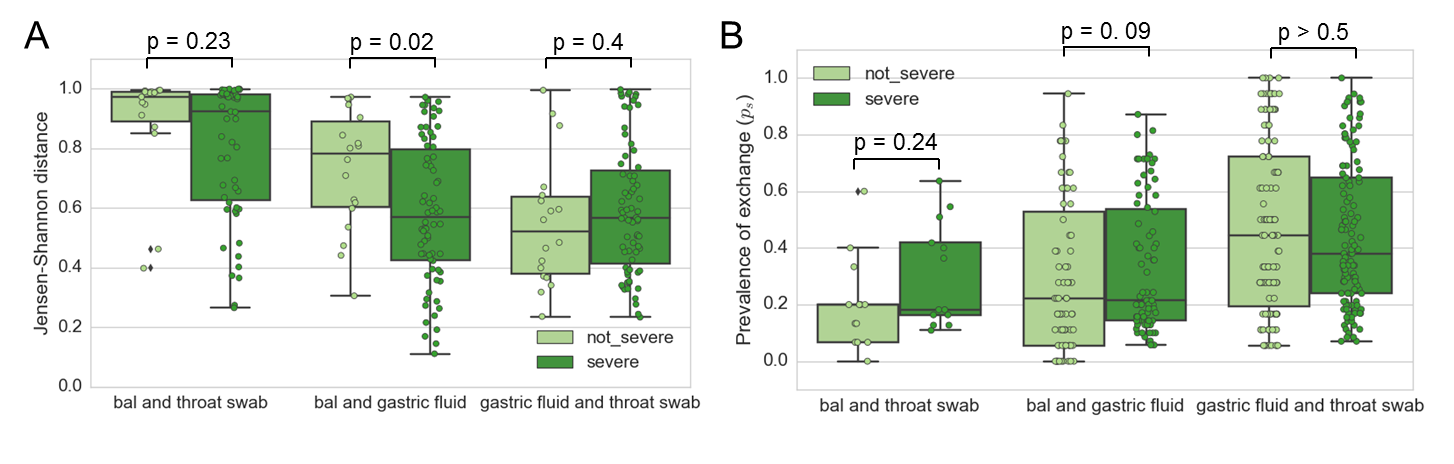
\includegraphics[scale=0.65]{reflux}
	\caption{Community similarities and exchange across sites, stratitified by reflux severity.
	(A) and (B) as in Figure \ref{fig:similarities}.}
	\label{fig:reflux}
\end{center}
\end{figure}


\subsection{Aim 2: Meta-analysis of gut microbiome studies}

\subsubsection{Collect and process 16S case-control datasets}
Our literature review has identified over 50 suitable case-control 16S datasets,
28 of which have been downloaded with associated metadata and processed through our in-house pipeline.
Characteristics of these datasets, including sample size, disease states,
and median sequencing depth, are shown in Appendix \ref{sec:appendix_tables}, Table \ref{tab:datasets}.

\subsubsection{General microbial signature of diseases is especially apparent in diarrheal diseases}
We first summarized overall community structure using Shannon's alpha diversity
index (SDI). As expected, we observed significant batch effects across studies, likely due to
the differences in sequencing depth (Appendix \ref{sec:appendix_figures}, Figure \ref{fig:alpha_all}). After standardizing SDI within studies
and combining similar disease states, we observed little difference in overall
community structure between cases and controls. An exception to this was seen
in diarrheal diseases (\textit{Clostridium difficile} infection and enteric 
diarrheal disease), in which alpha diversity was significantly lower in the cases (Figure \ref{fig:alpha}). Interestingly, disease states which had multiple studies that defined
their cases or controls differently also showed significant differences
in alpha diversity. For example, one IBD study \cite{ibd-papa} recruited controls
with non-inflammatory conditions of the gastrointestinal tract while others \cite{ibd-gevers, ibd-engstrand, ibd_hut}
used healthy patients as controls. Additionally, some obesity studies \cite{ob-escobar, ob-goodrich, ob-gordon} labeled patients as ``overweight'' in addition
to ``obese'' while others \cite{ob-ross, ob-zupancic} included only ``healthy'' and ``obese'' patient 
category labels. These cases were the only non-diarrheal significant
differences in alpha diversity and were less striking than the differences in
diarrheal disease, and are 
hypothesized to be driven by batch effects rather than biology.
Further work to investigate this hypothesis will involve applying 
different standardization techniques and including the 
individual studies as factors in the statistical comparisons across cohorts.

\begin{figure}
\begin{center}
	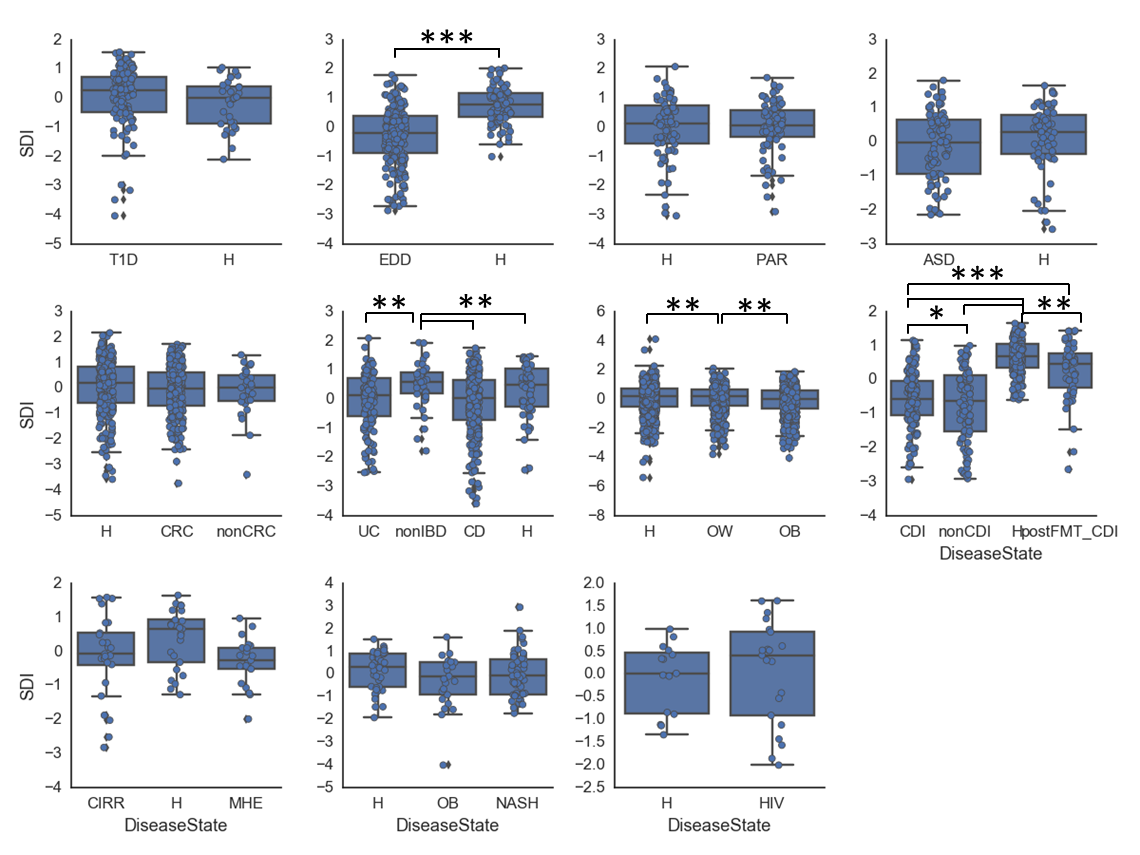
\includegraphics[scale=0.55]{alpha_diversity_by_study_type}
	\caption{Alpha diversity by study type. Q-values calculated by independent t-tests and corrected for Benjamini-Hochberg false discovery rate. $q \approx 0$ (***), $q \textless 0.0001$ (**), $q \textless 0.01$ (*)}	\label{fig:alpha}
\end{center}
\end{figure}

We next performed within-study univariate comparisons of genus level-abundances in cases vs. controls. Diarrheal 
diseases had striking shifts in many microbes, while other
diseases had less obviously apparent microbial indicators of disease (Appendix \ref{sec:appendix_figures}, Figure \ref{fig:larger_pval_heatmap}). We also observed that some bacteria
seemed to have relatively consistent shifts across many
different diseases. We confirmed the significance of these associations by combining the p-values of each genus across all studies using the weighted Z-test method \cite{zavkin-ztest-2011}.
We found many genera in the family \textit{Enterobacteriaceae} to be associated
with disease in general, while many genera in the families \textit{Lachnospiraceae}, 
and \textit{Ruminococcaceae} were associated with healthy controls.
These results support the hypothesis that
there is a general signature for disease, in other words, that sick people have 
altered microbiomes. In light of this finding, focusing on microbial shifts that 
are unique to individual diseases will be crucial to identify disease-specific biomarkers
that could be used for diagnostic purposes and to motivate future mechanistic investigations of microbial interactions with disease.

%\newpage
%\begin{figure}[h]
%	\begin{center}
%  	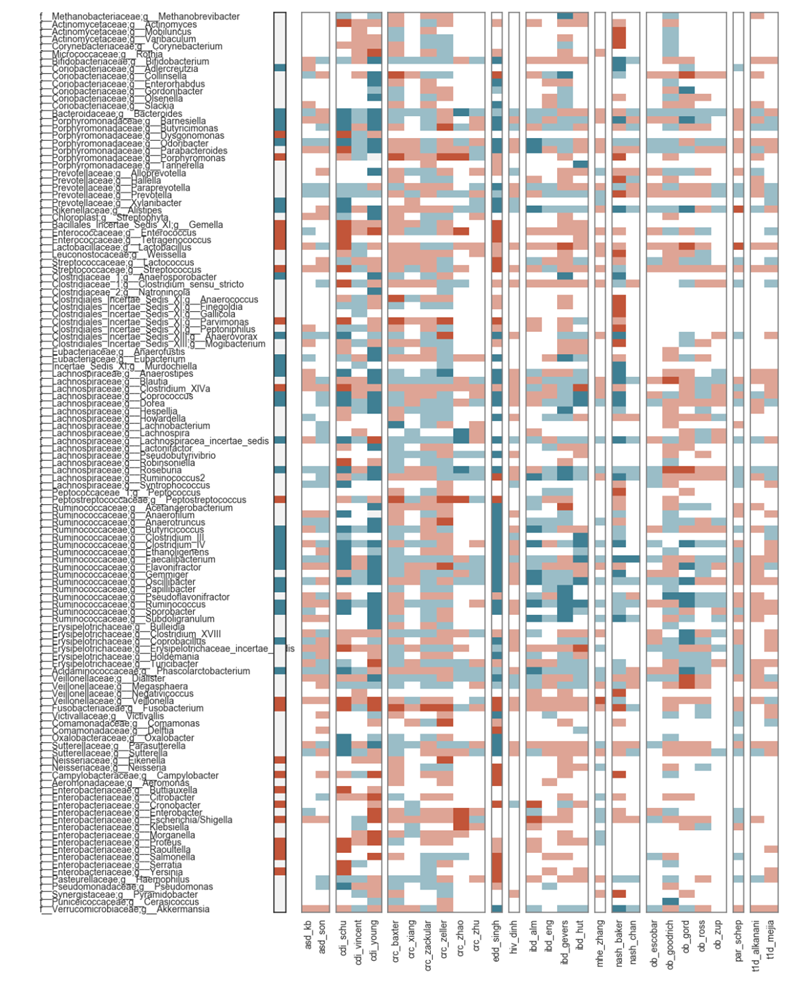
\includegraphics[scale=0.95]{pval_heatmap}
%	\caption{}
%	\label{fig:pval_heatmap}
%	\end{center}
%\end{figure}

\newpage
\section{Appendix}
\subsection{Supplementary Tables}\label{sec:appendix_tables}

{
\renewcommand{\arraystretch}{1.1}
\begin{table}[h]
\resizebox{\textwidth}{!}{\begin{tabular}{|c|c|c|c|c|c|c|c|c|}
	\hline
	\textbf{Dataset ID} & \textbf{Year} & \textbf{Disease(s)} &	\textbf{N control} & \textbf{N case} & \parbox[c]{2cm}{\centering\textbf{Median}\\\textbf{reads per}\\\textbf{sample}} &	\textbf{Sequencer} & \textbf{16S Region} & \textbf{Ref.} \\
	\hline
	asd\_kb & 2013 & ASD & 20 & 19 & 1345 & 454 & V2-V3 & \cite{asd-kb}\\ 
	asd\_son & 2015 & ASD & 44 & 59 & 4777 & Miseq & V1-V2  & \cite{asd-son}\\ 
	cdi\_schu & 2014 & CDI & 243 & 93 & 3557 & 454 & V3-V5 & \cite{cdi_schubert}\\ 
	cdi\_vincent & 2013 & CDI & 18 & 17 & 5518 & 454 & V1-V3 & \cite{cdi_vincent}\\ 
	cdi\_young & 2014 & CDI & 18 & 27 & 16516 & Miseq & V4 & \cite{cdi_youngster}\\ 
	crc\_baxter & 2016 & CRC & 122 & 120 & 9476 & Miseq & V4 & \cite{crc_baxter}\\ 
	crc\_xiang & 2012 & CRC & 22 & 21 & 1152 & 454 & V1-V3 & \cite{crc_xiang}\\ 
	crc\_zackular & 2014 & CRC & 58 & 30 & 54269 & MiSeq & V4 & \cite{crc_zackular}\\ 
	crc\_zeller & 2014 & CRC & 75 & 41 & 120612 & MiSeq & V4 & \cite{crc_zeller}\\ 
	crc\_zhao & 2012 & CRC & 54 & 44 & 161 & 454 & V3 & \cite{crc_zhao}\\ 
	crc\_zhu & 2013 & CRC & 18 & 12 & 1835 & 454 & V3 & \cite{crc_zhu}\\ 
	edd\_singh & 2015 & EDD & 82 & 222 & 2573 & 454 & V3-V5 & \cite{edd-singh}\\ 
	hiv\_dinh & 2015 & HIV & 15 & 21 & 3248 & 454 & V3-V5 & \cite{hiv-dinh}\\ 
	ibd\_alm & 2012 & UC, CD & 24 & 66 & 1303 & 454 & V3-V5 & \cite{ibd-papa}\\ 
	ibd\_eng & 2009 & UC, CD & 32 & 32 & 2658 & 454 & V5-V6 & \cite{ibd-engstrand}\\ 
	ibd\_gevers & 2014 & CD & 16 & 146 & 9773 & Miseq & V4 & \cite{ibd-gevers}\\ 
	ibd\_hut & 2012 & UC, CD & 27 & 186 & 995 & 454 & V3-V5 & \cite{ibd_hut}\\ 
	mhe\_zhang & 2013 & CIRR, MHE & 25 & 46 & 487 & 454 & V1-V2 & \cite{mhe_zhang}\\ 
	nash\_baker & 2013 & NASH, OB & 16 & 47 & 9904 & 454 &   & \cite{nash-baker}\\ 
	nash\_chan & 2013 & NASH & 22 & 32 & 1743 & 454 & V1-V2 & \cite{nash-chan}\\ 
	ob\_escobar & 2014 & OW, OB & 10 & 20 & 1126 & 454 & V1-V3 & \cite{ob-escobar}\\ 
	ob\_goodrich & 2014 & OW, OB & 451 & 528 & 27364 & Miseq & V4 & \cite{ob-goodrich}\\ 
	ob\_gord & 2009 & OW, OB & 61 & 219 & 1569 & 454 & V2 & \cite{ob-gordon}\\ 
	ob\_ross & 2015 & OB & 26 & 37 & 1583 & 454 & V1-V3 & \cite{ob-ross}\\ 
	ob\_zup & 2012 & OB & 167 & 117 & 1392 & 454 & V1-V3 & \cite{ob-zupancic}\\ 
	par\_schep & 2015 & PAR & 74 & 74 & 2351 & 454 & V1-V3 & \cite{par-schep}\\ 
	t1d\_alkanani & 2015 & T1D & 23 & 89 & 9117 & MiSeq & V4 & \cite{t1d_alkanani}\\ 
	t1d\_mejia & 2014 & T1D & 8 & 21 & 4702 & 454 & V3-V5 & \cite{t1d_mejia}\\ 	
	\hline
\end{tabular}}
\caption{Datasets currently collected and processed through standardized pipeline. Disease labels: ASD = Austism spectrum disorder, CDI = \textit{Clostridium difficile} infection, CRC = colorectal cancer, EDD = enteric diarrheal disease, UC = Ulcerative colitis, CD = Crohn's disease, CIRR = Liver cirrhosis, MHE =  minimal hepatic encephalopathy, NASH = non-alcoholic steatohepatitis, OW = overweight, OB = obese, PAR = Parkinson's disease, T1D = Type I Diabetes. }\label{tab:datasets}
\end{table}
}

\newpage
\subsection{Supplementary Figures}\label{sec:appendix_figures}

\begin{figure}[h]
\begin{center}
	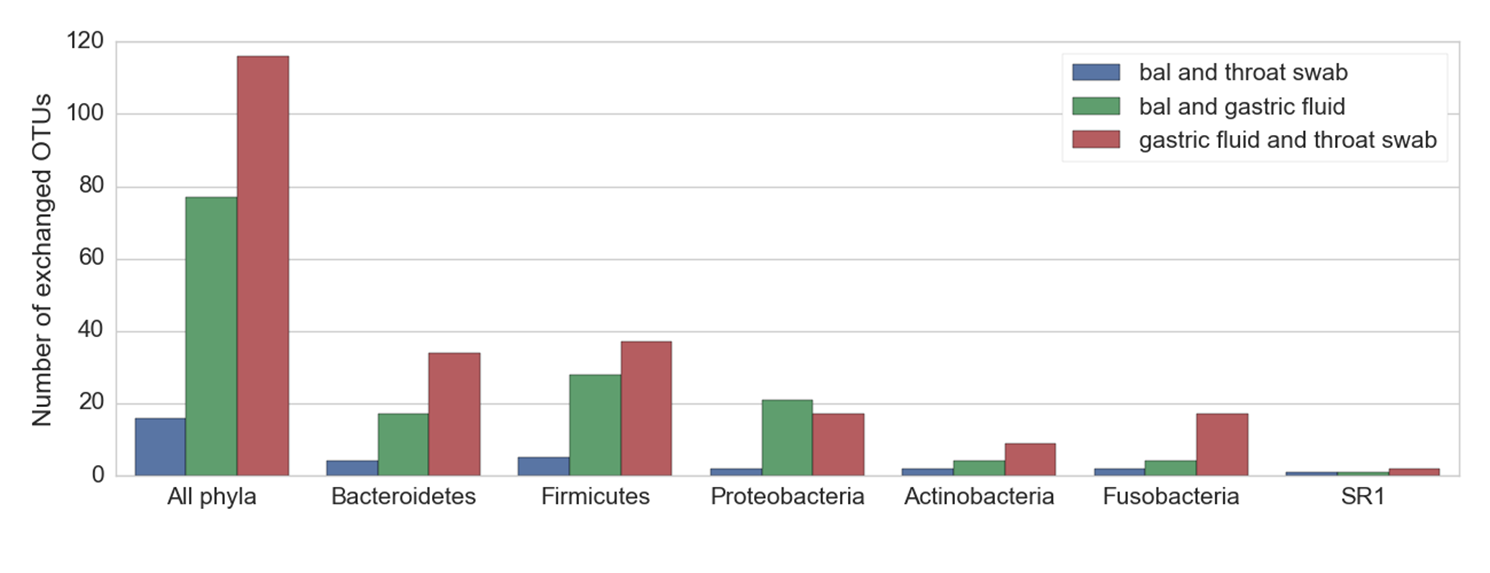
\includegraphics[scale=0.6]{shared_phyla}
	\caption{Number of exchanged OTUs across aerodigestive tract
	sites, separated by phyla.}
	\label{fig:shared_phyla}
\end{center}
\end{figure}

\newpage

%\begin{figure}[h]
%	\begin{center}
%  	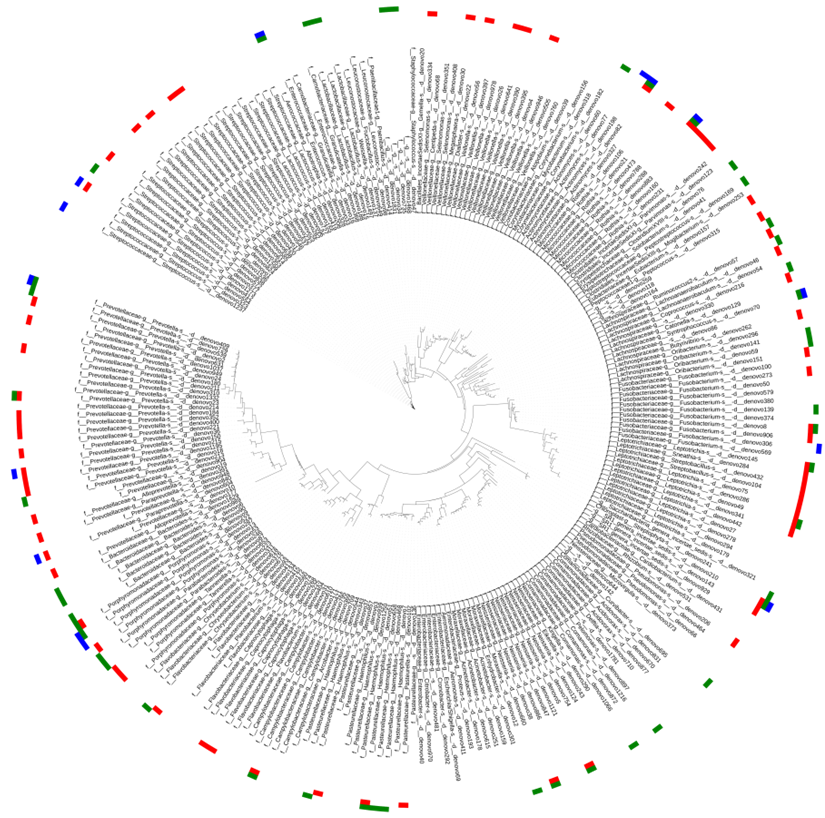
\includegraphics[scale=1.1]{rosen_tree}
%	\caption{Phylogenetic tree built on 99\% OTUs and labeled based on their
%	exchange across aerodigestive tract sites
%	(red = throat and gastric, green = gastric and lungs, blue = 
%	throat and lungs). Tree visualized with iTOL \cite{letunic-itol-2016}.}
%	\label{fig:rosen_tree}
%	\end{center}
%\end{figure}

\newpage
\begin{figure}[h]
\begin{center}
	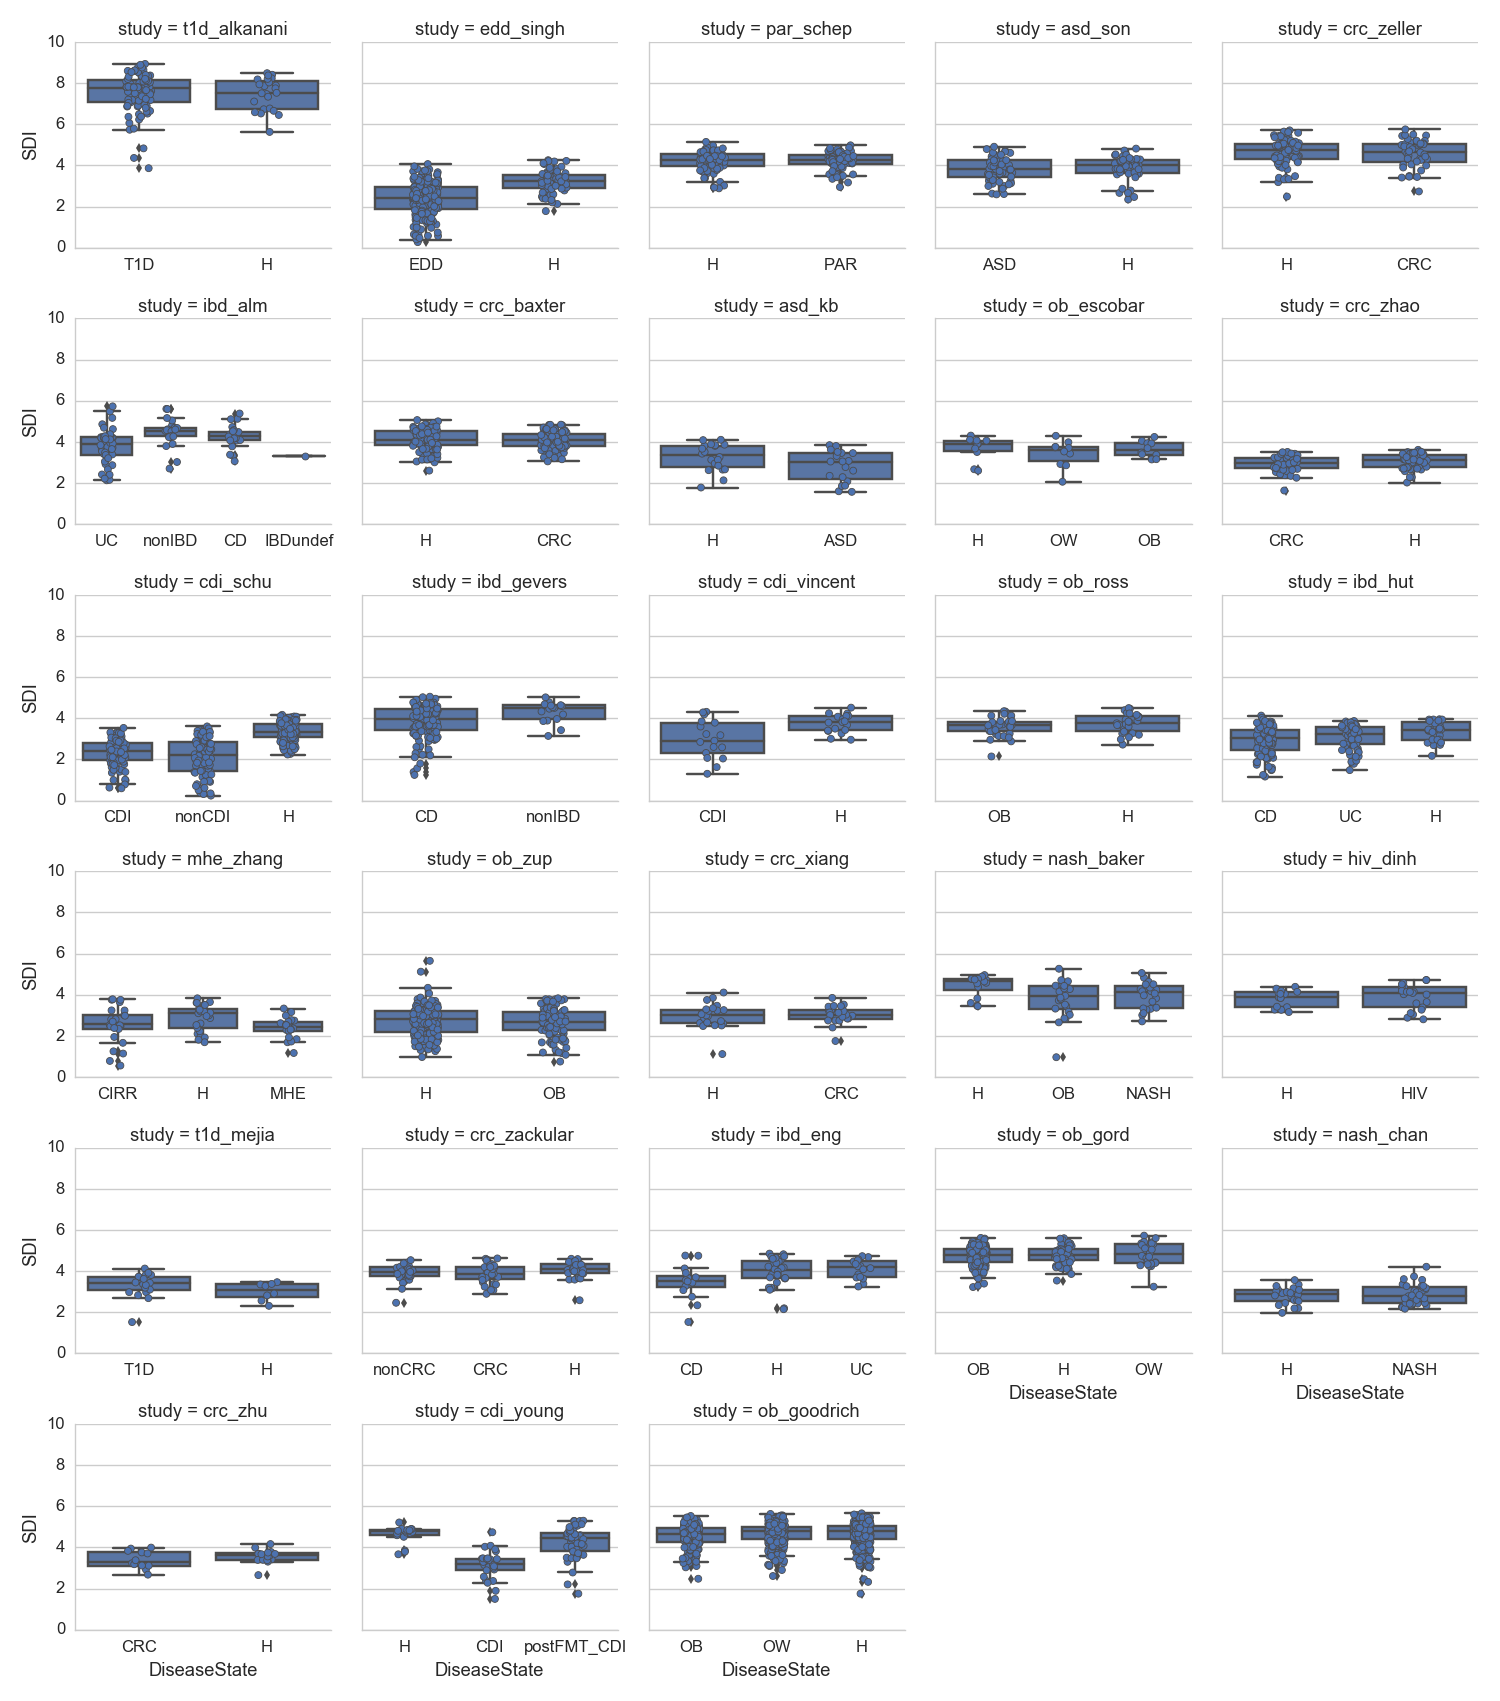
\includegraphics[scale=0.45]{alpha_diversity_by_study}
	\caption{Shannon alpha diversity index (SDI), stratified by individual studies. Note how the range of SDI varies across studies.}
	\label{fig:alpha_all}
\end{center}
\end{figure}

\newpage
\begin{figure}[h]
	\begin{center}
  	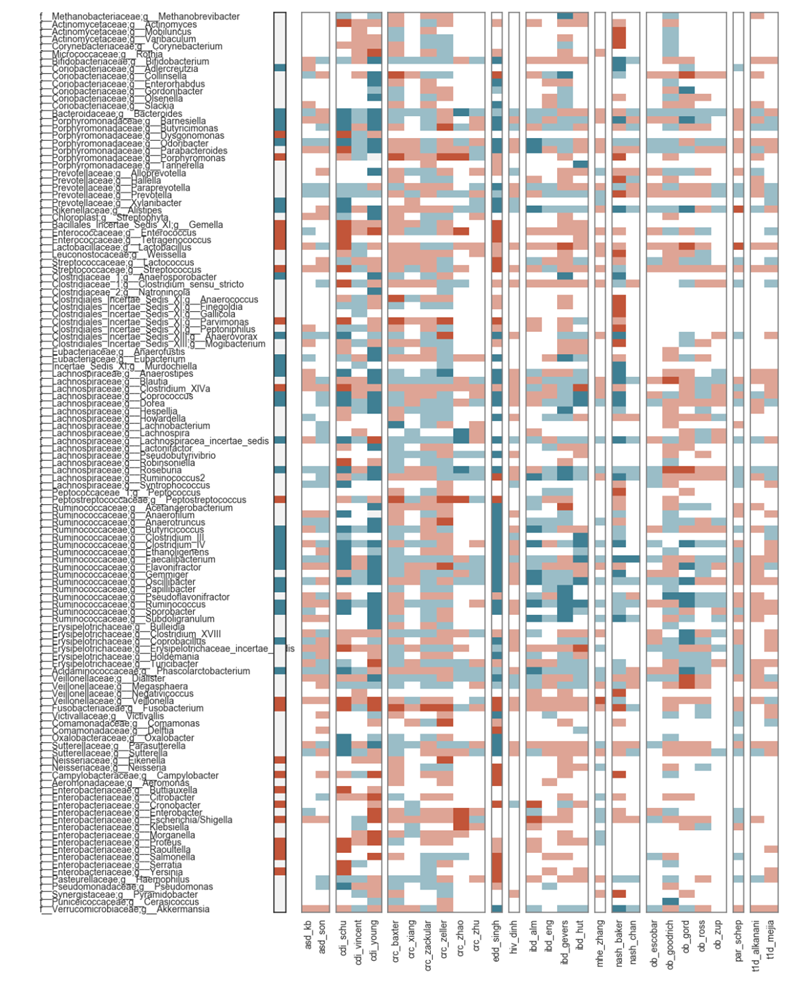
\includegraphics[scale=1.2]{pval_heatmap}
	\caption{Heatmap of genus-level associations with disease across all
	compiled studies. Color indicates whether the mean abundance of the organism
	was higher in the control patients (blue) or disease (red). Shade indicates
	whether the association was significant after FDR correction (dark color) or not
	significant (light color), $\alpha = 0.05$. Genus associations which were 
	significant	after combining q-values across all studies are shown in the bar to 	
	the left of the heatmap. Studies are labeled along the x-axis and described in
	Appendix \ref{sec:appendix_tables}, Table \ref{tab:datasets}; genera are labeled 
	along the y-axis.}
	\label{fig:larger_pval_heatmap}
	\end{center}
\end{figure}

\FloatBarrier

\newpage


\bibliographystyle{unsrtnat}
\bibliography{refs}

\end{document}